\documentclass[greek]{beamer}
%\usepackage{fontspec}
\usepackage{amsmath,amsthm}
\usepackage{unicode-math}
\usepackage{xltxtra}
\usepackage{graphicx}
\usetheme{CambridgeUS}
\usecolortheme{seagull}
\usepackage{hyperref}
\usepackage{ulem}
\usepackage{xgreek}

\usepackage{pgfpages} 
\usepackage{tikz}
%\setbeameroption{show notes on second screen}
%\setbeameroption{show only notes}

\setsansfont{Calibri}

\usepackage{multicol}

\usepackage{appendixnumberbeamer}

\usepackage{polynom}

\usepackage{pgffor}

\setbeamercovered{transparent}
\beamertemplatenavigationsymbolsempty

\title{Συναρτήσεις}
\subtitle{Μονοτονία}
\author[Λόλας]{Κωνσταντίνος Λόλας }
\institute[$10^ο$ ΓΕΛ]{$10^ο$ ΓΕΛ Θεσσαλονίκης}
\date{}

\begin{document}

\begin{frame}
      \titlepage
\end{frame}
\begin{frame}{Μονοτονία Συναρτήσεων}
      \begin{block}{Ορισμός}
            Μία συνάρτηση $f$ είναι \emph{γνησίως αύξουσα} σε ένα διάστημα $Δ$ αν
            $$\text{για κάθε } x_1,x_2\in Δ \text{ με } x_1<x_2\implies f(x_1)<f(x_2)$$
      \end{block} \pause
      \begin{block}{Ορισμός}
            Μία συνάρτηση $f$ είναι \emph{γνησίως φθίνουσα} σε ένα διάστημα $Δ$ αν
            $$\text{για κάθε } x_1,x_2\in Δ \text{ με } x_1<x_2\implies f(x_1)>f(x_2)$$
      \end{block}
\end{frame}

\begin{frame}{Ποιός δεν αναρωτιέται?}
      Ισχύει η συνεπαγωγή για έστω μια γνησίως αύξουσα
      $$x_1<x_2\iff f(x_1)<f(x_2)$$
      \only<1>{?} \pause
      Φυσικά (?)
\end{frame}

\begin{frame}{αύξουσα, σκέτο αύξουσα}
      \begin{block}{Ορισμός}
            Μία συνάρτηση $f$ είναι \emph{αύξουσα} σε ένα διάστημα $Δ$ αν
            $$\text{για κάθε } x_1,x_2\in Δ \text{ με } x_1<x_2\implies f(x_1)\le f(x_2)$$
      \end{block} \pause
      \begin{block}{Ορισμός}
            Μία συνάρτηση $f$ είναι \emph{φθίνουσα} σε ένα διάστημα $Δ$ αν
            $$\text{για κάθε } x_1,x_2\in Δ \text{ με } x_1<x_2\implies f(x_1)\ge f(x_2)$$
      \end{block}
\end{frame}

\begin{frame}{Συγκρατήσαμε τίποτα?}
      \begin{exampleblock}{Παραδείγματα}
            \begin{itemize}
                  \item $f(x)=x^2$ \pause
                  \item $f(x)=1/x$
            \end{itemize}
      \end{exampleblock}
\end{frame}

\begin{frame}{Οι ελέφαντες θυμούνται, εσείς?}
      Γράψτε στο τετράδιο όσες γνησίως αύξουσες συναρτήσεις θυμάστε \pause
      \begin{multicols}{2}
            \begin{itemize}
                  \item $ax+b$, $a>0$
                  \item $\ln x$
                  \item $x^2$, $x\ge 0$
                  \item $x^3$
                  \item $e^x$, $2^x$
                  \item $ημ x$, $0< x< \pi/2$
                  \item $εφ x$
            \end{itemize} \pause
      \end{multicols}

      Γράψτε στο τετράδιο όσες γνησίως φθίνουσες συναρτήσεις θυμάστε \pause
      \begin{multicols}{2}
            \begin{itemize}
                  \item $ax+b$, $a<0$
                  \item $x^2$, $x\le 0$
                  \item $-x^3$
                  \item $\left(\frac{1}{2}\right)^x$, $e^{-x}$
                  \item $συν x$, $0< x< \pi/2$
                  \item $\frac{1}{x}$, $x<0$
            \end{itemize}
      \end{multicols}
\end{frame}

\begin{frame}{Μπρίκια κολάμε?}
      Θα ασχολούμαστε
      \begin{itemize}
            \item με κατασκευές
            \item ανισώσεις
      \end{itemize}
\end{frame}

\section{Ασκήσεις}

\subsection{Άσκηση 1}
\begin{frame}[label=Άσκηση1,t]{Εξάσκηση 1}
      Η συνάρτηση $f$ του σχήματος είναι ορισμένη στους πραγματικούς αριθμούς.
      \begin{itemize}
            \item Να γράψετε τα διαστήματα μονοτονίας της
            \item Να συγκρίνετε τις τιμές
                  \begin{itemize}
                        \item $f(2)$ και $f(e)$
                        \item $f(3)$ και $f(\pi)$
                  \end{itemize}
      \end{itemize}
      \centering
      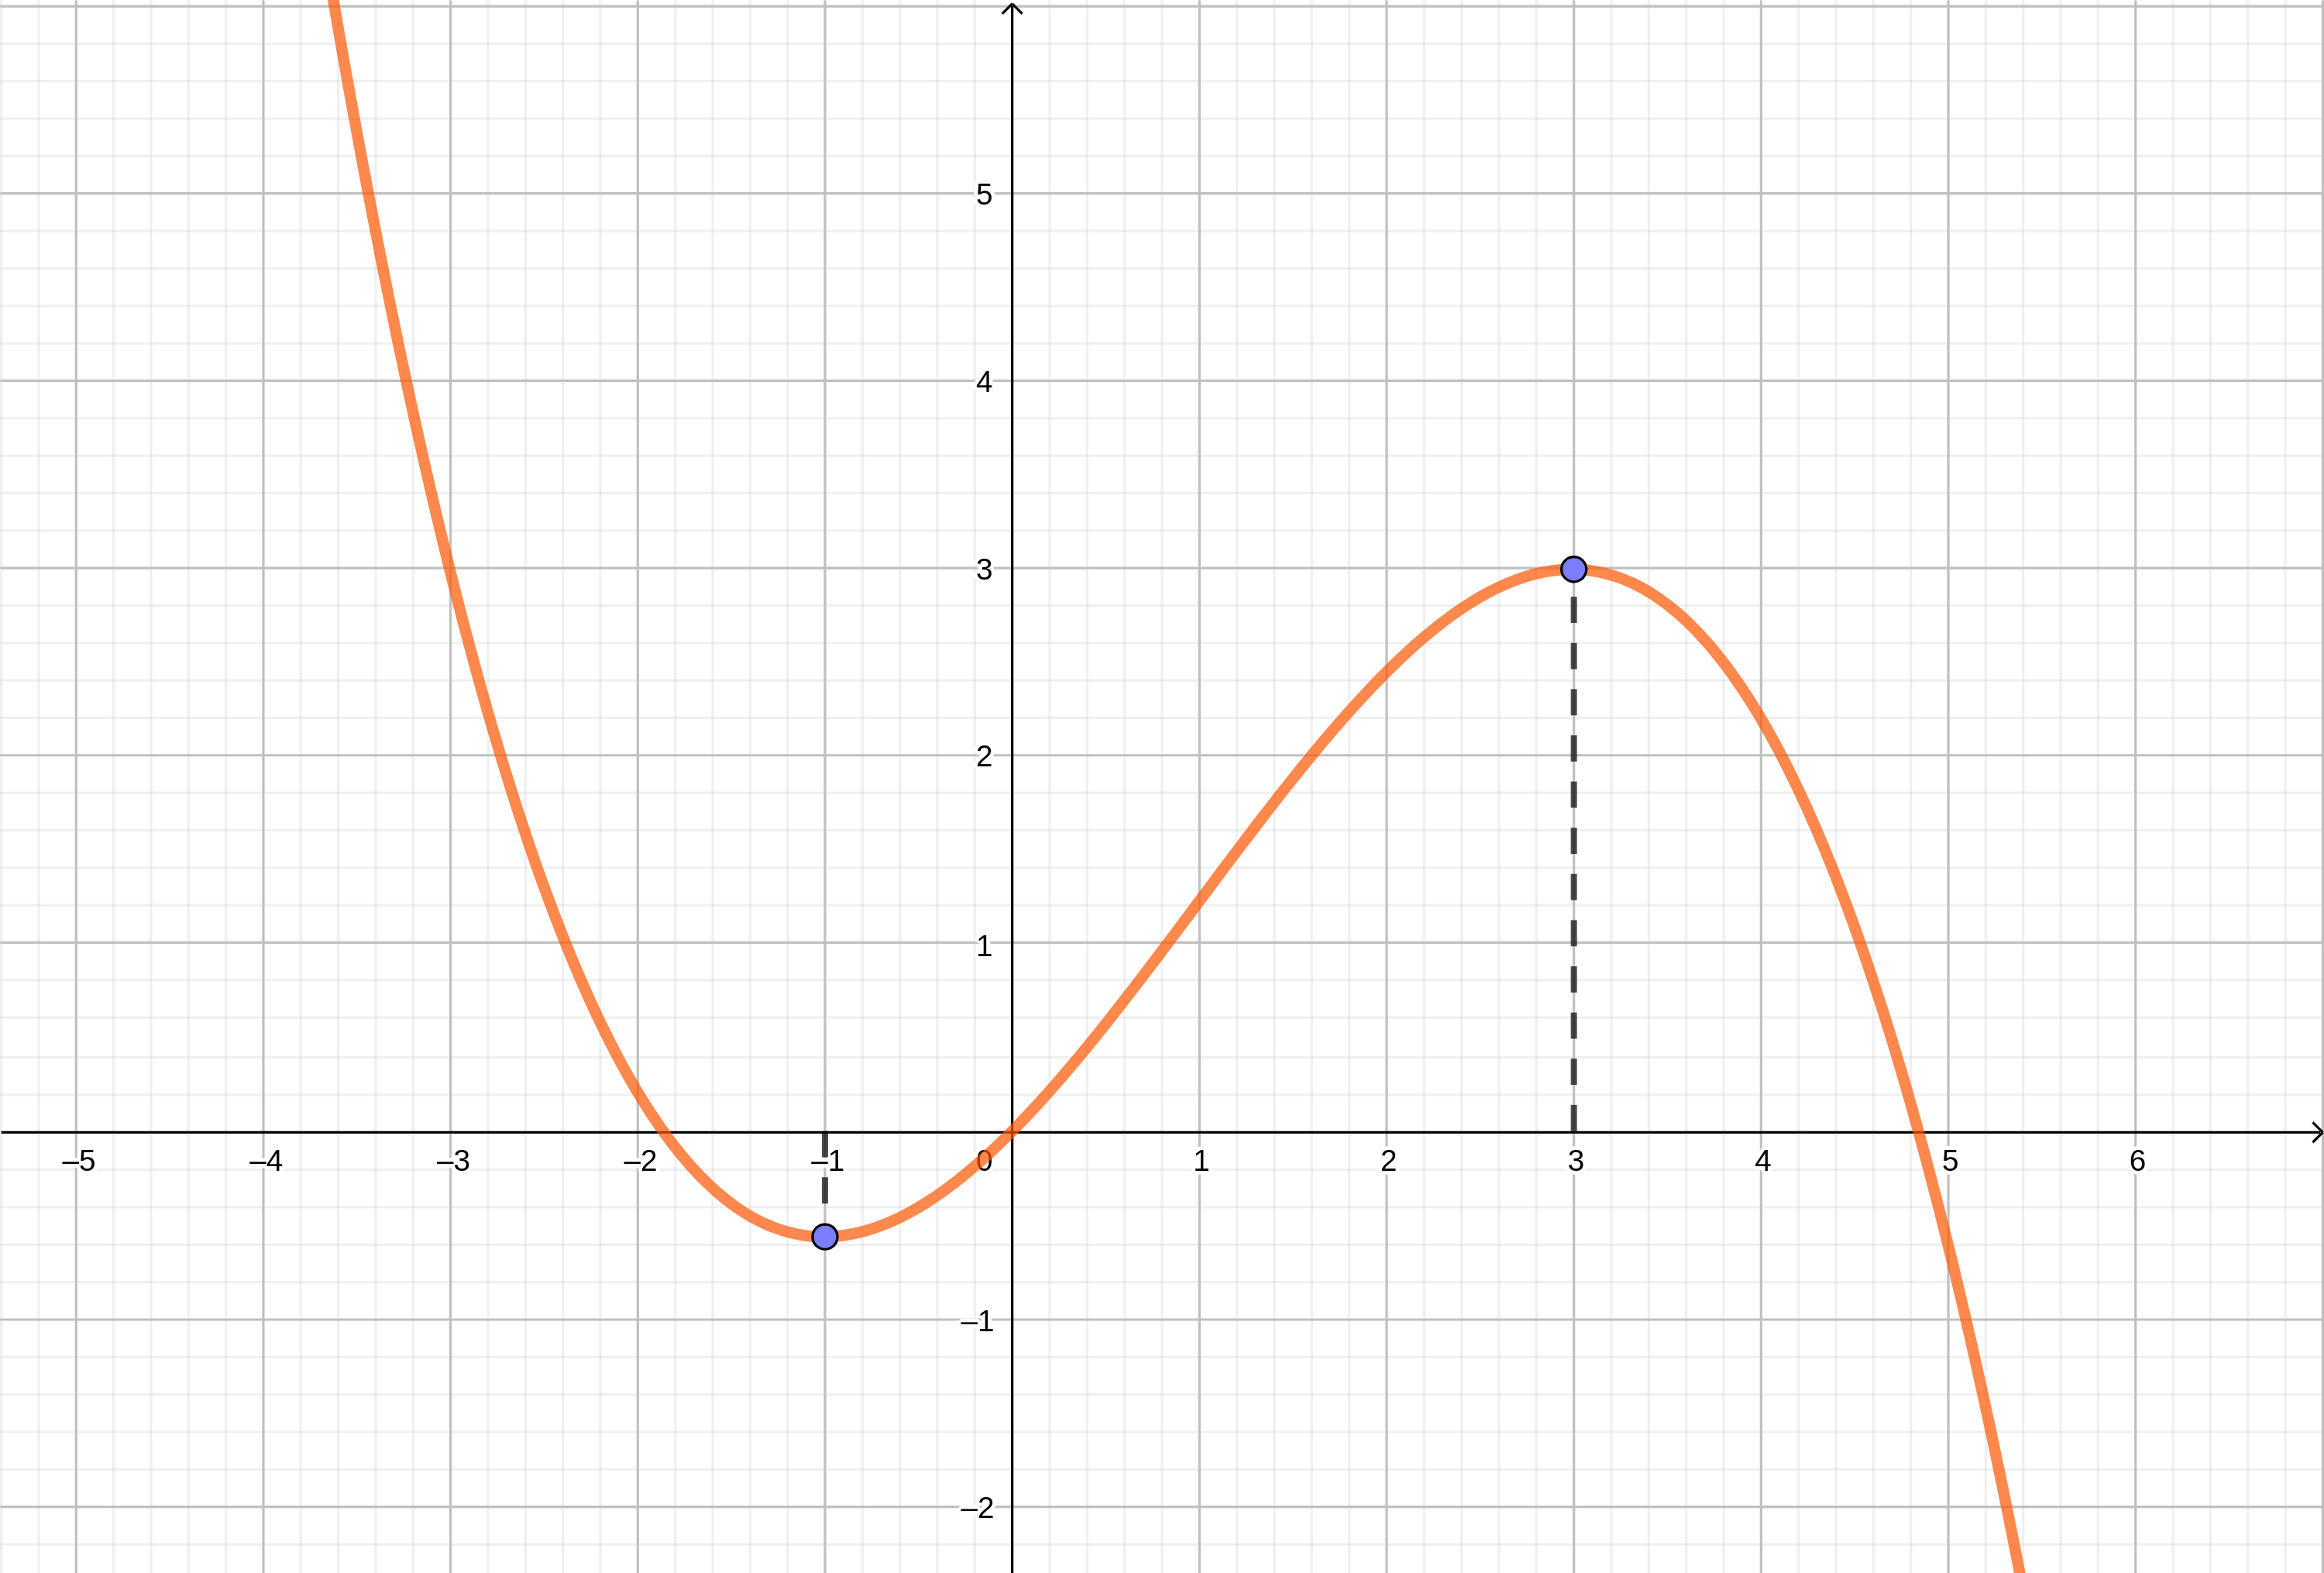
\includegraphics[width=0.5\textwidth]{"images/1.3 Μονοτονία.png"}
\end{frame}

\subsection{Άσκηση 2}
\begin{frame}[label=Άσκηση2,t]{Εξάσκηση 2}
      Δίνεται η συνάρτηση $f(x)=x^3+3x-5$
      \begin{enumerate}
            \item Να μελετήσετε την συνάρτηση ως προς την μονοτονία \pause
            \item Να συγκρίνετε τις τιμές $f(2022)$ και $f(2023)$
      \end{enumerate}
\end{frame}

\subsection{Άσκηση 3}
\begin{frame}[label=Άσκηση3,t]{Εξάσκηση 3}
      Δίνεται η συνάρτηση $f(x)=e^x+\ln x-1$
      \begin{enumerate}
            \item Να μελετήσετε την συνάρτηση ως προς την μονοτονία \pause
            \item Να αποδείξετε ότι:
                  \begin{enumerate}
                        \item Αν $x>1$, τότε $e^x+\ln x>e$ \pause
                        \item Αν $α$, $β>0$ και $α<β$, τότε $\ln \frac{α}{β}<e^β-e^α$ \pause
                        \item Για κάθε $x>0$, $f(x+1)-f(x)>0$ \pause
                        \item Για κάθε $x>0$, $f(x)<f(2x)$ \pause
                        \item Για κάθε $x>1$, $f(x^2)>f(x)$
                  \end{enumerate}
      \end{enumerate}
\end{frame}

\subsection{Άσκηση 4}
\begin{frame}[label=Άσκηση4,t]{Εξάσκηση 4}
      \begin{enumerate}
            \item Να βρείτε τις ρίζες και το πρόσημο της συνάρτησης $f(x)=e^x+2x-1$ \pause
            \item Να βρείτε το πεδίο ορισμού των συναρτήσεων:
                  \begin{enumerate}
                        \item $g(x)=\ln f(x)$ \pause
                        \item $h(x)=\frac{1}{f(x)}$
                  \end{enumerate}
      \end{enumerate}
\end{frame}

\subsection{Άσκηση 5}
\begin{frame}[label=Άσκηση5,t]{Εξάσκηση 5}
      Έστω $f:\mathbb{R}\to\mathbb{R}$ μία συνάρτηση, η οποία είναι γνησίως φθίνουσα. Να λύσετε τις ανισώσεις:
      \begin{itemize}
            \item $f(x)>f(3)$
            \item $f(2x+1)<5$, αν $f(3)=5$
            \item $f(x^2-3x)\ge f(2-4x)$
            \item $f\left(f(3x-1)\right)<f\left(f(2x+3)\right)$
      \end{itemize}
\end{frame}

\subsection{Άσκηση 6}
\begin{frame}[label=Άσκηση6,t]{Εξάσκηση 7}
      Δίνεται η συνάρτηση $f(x)=e^x+x-1$
      \begin{enumerate}
            \item Να μελετήσετε την συνάρτηση ως προς την μονοτονία \pause
            \item Να λύσετε τις ανισώσεις:
                  \begin{enumerate}
                        \item $f(x)>0$ \pause
                        \item $e^x+x<e+1$ \pause
                        \item $f(e^x+x+1)>1+e^2$ \pause
                        \item $e^{f(x)}+f(x)-x>e^x$
                  \end{enumerate}
      \end{enumerate}
\end{frame}

\subsection{Άσκηση 7}
\begin{frame}[label=Άσκηση7,t]{Εξάσκηση 7}
      Δίνεται η συνάρτηση $f(x)=x^5+x-2$. Να λύσετε τις ανισώσεις:
      \begin{enumerate}
            \item $x<\frac{2}{x^4+1}$ \pause
            \item $x^4-\frac{2}{x}>-1$, στο $(0,+\infty)$ \pause
            \item $\ln^5 x+\ln x<2$ \pause
            \item $f(2x-1)+2>x^5+x$
      \end{enumerate}
\end{frame}

\subsection{Άσκηση 8}
\begin{frame}[label=Άσκηση8,t]{Εξάσκηση 8}
      Δίνεται η συνάρτηση $f(x)=x+\ln (x+1)$
      \begin{enumerate}
            \item Να εξετάσετε τη συνάρτηση $f$ ως προς τη μονοτονία \pause
            \item Να λύσετε την ανίσωση $x^2+\ln (x^2+1)>0$ \pause
            \item Να λύσετε την ανίσωση $x^4-x^2<\ln \frac{x^2+1}{x^4+1}$
      \end{enumerate}
\end{frame}

\subsection{Άσκηση 9}
\begin{frame}[label=Άσκηση9,t]{Εξάσκηση 9}
      Να λύσετε τις ανισώσεις:
      \begin{enumerate}
            \item $e^x+x^3<1$ \pause
            \item $e^x-e^{x^2}>\ln x$
      \end{enumerate}
\end{frame}

\subsection{Άσκηση 10}
\begin{frame}[label=Άσκηση10,t]{Εξάσκηση 10}
      Έστω $f:\mathbb{R}\to\mathbb{R}$ μία συνάρτηση με $f(0)=1$ και $f\uparrow$. Να λύσετε τις ανισώσεις:
      \begin{enumerate}
            \item $f(x)+e^x>2$ \pause
            \item $(x+1)f(x)<1$, στο $(-1,+\infty)$
      \end{enumerate}
\end{frame}

\subsection{Άσκηση 11}
\begin{frame}[label=Άσκηση11,t]{Εξάσκηση 11}
      Δίνονται οι συναρτήσεις $f(x)=e^x$, $x>0$ και $g(x)=\frac{e}{x}$, $x>0$.
      \begin{enumerate}
            \item Να βρείτε τα κοινά σημεία των $C_f$ και $C_g$ \pause
            \item Να βρείτε τη σχετική θέση των $C_f$ και $C_g$
      \end{enumerate}
\end{frame}

\subsection{Άσκηση 12}
\begin{frame}[label=Άσκηση12,t]{Εξάσκηση 12}
      Έστω $g:(0,+\infty)\to\mathbb{R}$ μία γνησίως μονότονη συνάρτηση της οποίας η γραφική παράσταση διέρχεται από τα σημεία $Α(1,-2)$, $Β(2,-3)$ και η συνάρτηση $f(x)=\ln x-g(x)$, $x>0$.
      \begin{enumerate}
            \item Να δείξετε ότι η $g$ είναι γνησίως φθίνουσα \pause
            \item Να δείξετε ότι η $f$ είναι γνησίως αύξουσα \pause
            \item Να λύσετε την ανίσωση $2\ln x<2+g(x^2)$
      \end{enumerate}
\end{frame}

\subsection{Άσκηση 13}
\begin{frame}[label=Άσκηση13,t]{Εξάσκηση 13}
      Έστω $f,g:\mathbb{R}\to\mathbb{R}$ δύο συναρτήσεις με $g\uparrow$ και
      $$g(x)=f(x+1)-f(x)\text{, για κάθε } x\in\mathbb{R}$$
      \begin{enumerate}
            \item Να λύσετε τις ανισώσεις
                  \begin{enumerate}
                        \item $f(\ln x+1)>f(\ln x)$, αν $f(1)=f(2)$ \pause
                        \item $f(\sqrt{x}+1)f(x+1)<f(\sqrt{x})-f(x)$ \pause
                  \end{enumerate}
            \item Να αποδείξετε ότι  \pause
                  $$f(e^x+1)-f(ημ x+1)>f(e^x)-f(ημ x)\text{, για κάθε } x>0$$
      \end{enumerate}
\end{frame}

\subsection{Άσκηση 14}
\begin{frame}[label=Άσκηση14,t]{Εξάσκηση 14}
      Έστω $f:\mathbb{R}\to\mathbb{R}$ μία συνάρτηση η οποία είναι γνησίως φθίνουσα
      \begin{enumerate}
            \item Να δείξετε ότι $f(x)+f(7x)>f(3x)+f(10x)$, για κάθε $x>0$ \pause
            \item Να λύσετε την εξίσωση $f(x)+f(x^3)=f(x^2)+f(x^8)$, στο $(0,+\infty)$
      \end{enumerate}
\end{frame}

\subsection{Άσκηση 15}
\begin{frame}[label=Άσκηση15]{Εξάσκηση 15}

      \begin{enumerate}
            \item Έστω $f,g:\mathbb{R}\to\mathbb{R}$ δύο συναρτήσεις όπου $g\circ f \downarrow$ και $g\uparrow$. Να δείξετε ότι $f\downarrow$ \pause
            \item Έστω $f:\mathbb{R}\to\mathbb{R}$ μία συνάρτηση για την οποία ισχύει:
                  $$f^3(x)+e^{f(x)}-e^{-x}-1=0\text{, για κάθε } x\in\mathbb{R}$$
                  Να εξετάσετε τη συνάρτηση $f$ ως προς τη μονοτνία
      \end{enumerate}
\end{frame}

\begin{frame}
      Στο moodle θα βρείτε τις ασκήσεις που πρέπει να κάνετε, όπως και αυτή τη παρουσίαση
\end{frame}

\end{document}
